\documentclass[letterpaper]{article} 
\usepackage[english]{babel}
\usepackage{natbib} 
\usepackage{sebajara}

\usepackage{longtable}
\usepackage{pdflscape}
\usepackage{booktabs}

\usepackage{algpseudocode}
\usepackage{algorithmicx}
\usepackage{algorithm}
\newcommand*\Let[2]{\State #1 $\gets$ #2}

\usepackage[margin=1.5in]{geometry}

\title{Tools for Stochastic Modelling of Gene Networks}

\author{Sebasti\'an Jaramillo-Riveri, \\
  {\it AIV Master Program, Universit\'{e} Paris Decartes, France}\\
  \href{mailto:sebajarar@gmail.com}{sebajarar@gmail.com}\\
  \\
  Supervisor: Yaakov Benenson,\\
  {\it Department of Biosystems Science and Engineering, ETH, Switzerland}
}

\begin{document}
\maketitle
%\pagestyle{empty}
%\oddsidemargin = 0pt

\abstract{
  For Synthetic Biology to become a standard engineering
  discipline, predictive strategies for the design and optimisation of
  synthetic genetic circuits are critical\citep{Benenson2012a}. Due to the complexity of
  biological systems and the many possible combinations, theoretical
  modelling is needed. Particular is the case of mammalian systems
  known for their stochasticity\citep{Suter2011,Bleris2011}. Furthermore, many laboratories rely
  on transient transfection, which makes gene copy numbers per cell
  highly variable.

  We have explored current methods for stochastic modelling of gene
  circuits, and implemented a pipeline for simulation of reaction
  models in MATLAB and C, compatible with SimBiology Toolbox. The
  implementation is based on the ``First Reaction Method'', chosen for
  its generality. To account for species with variable initial
  condition (such as gene copy numbers), the pipeline supports initial
  states sampled from marginal distributions constrained by
  correlations. The user can specify different kinds of simulations,
  parameter scans, and plotting options.

  We hope that these tools would be helpful in the design and
  optimisation of future synthetic circuits. Further work would
  include model validation, addition of alternative simulation
  approaches, parameter inference, improvement of user interface, and
  increase the efficiency of the implementation.
}

\tableofcontents

\section{Theoretical Background}

We should briefly introduced the theoretical background related to the
simulation of reaction based models. Many of these notes are based on
the course ``Computational System Biology, Stochastic Approaches'' by
M. Khammash.

\subsection{Deterministic Reaction Models}

In general, in the deterministic setting we deal with Ordinary
Differential Equations (ODEs) of the form
\begin{center}
  $\begin{array}{rcl} 
    \derwrtt{X_1} & = & f_1(X_1,\dots,X_n) \\
    & \dots & \\
    \derwrtt{X_n} & = & f_n(X_1,\dots,X_n) \\
    \end{array}$
\end{center}
where $X_i$ represent the concentration of a single chemical
specie. The functions $f_i$ is the derivative of the concentration, which
is a function of the system's state. Each reaction will contribute to the
derivative 
$$\derwrtt{X_i} = \sum_{j=1}^{\mathsf{M}}S_{ij} r_j(X_1,\dots,X_n) $$
where $S_{ij}$ is the stoichiometry of specie $X_i$ in reaction $j$,
and $r_j(X)$ is the rate of reaction $j$ as a function of the species
concentration.

We can classify chemical reactions into two kinds: \emph{elementary}
and \emph{complex}. Elementary reactions are thought to be the result of a single
collision event, for example $A \to B$, or $A + B \to C$. The rate
of these reactions can be formulated as
$$r_j = k_j\prod_{i}\parenthesis{X_i}^{S_{ij}}, S_{ij} > 0$$
meaning that is proportional to the product of all reactants (left
hand side of the reaction), elevated to their stochiometric
coefficient. This is the so called \emph{mass-action law}. For
example, the reaction $A + B \to C$ would have rate proportional to
$[A][B]$\footnote{We will use brackets to denote a specie
  concentration}.

Complex reactions are thought as a concatenation of more than one
elementary reaction, thus possibly having rate laws different from
mass action. The final function depends on the mechanism. Examples are
\emph{Michaelis-Menten} and \emph{Hill} equations.

It is important to notice that reaction rate constants are not
necessarily ``constant''.  Such parameters might in turn depend on
variables hidden to our model, that happen not to vary much in the
context the model was developed.  This ultimately depends on the
granularity of the model.  It is important to be aware of potential
dependencies, specially if we want to extrapolate the results of our
models.  For example, is common to find RNA synthesis rate constants
used for gene expression models. These depend on available RNA
polymerase and upstream regulatory sequences. In other contexts, such
as other cell lines, or different growth conditions, they may prove to
have different values.

\subsection{Stochastic Interpretation}

Conceptually, reactions are not continuous processes: each reaction
have a discrete number of events per time. And more, each event
modifies the system in discrete fashion. The stochastic interpretation
of a reaction model attemps to correct for these facts.

Instead of using concentrations, we will use species copy
numbers as our state space, and model reactions as stochastic events
that modify the system's state. We should assume \emph{well stirred}
conditions, meaning we will avoid any kind of spatial inhomogeneities
and diffusion processes. 

Let's call a vector with copy number of every specie in our model
$X(t) \in \Omega$. $X(t)$ is a random variable. We will be interested
in the probability of finding the system in state $\coolx$ at time $t$
given some initial state $\coolx_0$ and time $t_0$:
$$\coolp(\coolx,t|\coolx_0,t_0) = \Prob(X(t) = \coolx|X(t_0) = \coolx_0)$$
Each reaction (from a total of $\mathsf{M}$) is a possible event. We
will assume that the number of events in time is a \emph{Poisson
  Process}. The rate of the Poisson Process, meaning the average
number of events occurrences per unit of time, is called
\emph{propensity}, and is a function of the system's state
($a(\coolx)$).  Also, we will call $\nu$ a vector specifying how a
single event modify the state space.

Following the laws of probability we find that $\coolp(\coolx,t)$ is
governed by the following equation
$$\derwrtt{\coolp}(\coolx,t) = \sum_{j=1}^{\mathsf{M}} \brackets{a_j(\coolx - \nu_j)\coolp(\coolx - \nu_i,t) - a_j(\coolx)\coolp(\coolx,t)}$$
This is the so called Chemical Master Equation (CME). For convenience,
we have defined $\coolp(x,t)=0$, for all $x \notin \Omega$. Notice
that this equation gives an ODE that describes the evolution in time
of the \emph{p.m.f} for each possible state of the system, instead of
one ODE per specie as in the deterministic approach.

\subsection{Meso and Macro Scales}

In principle, if we were to divide the species states by the systems
volume $V$, we would recover species concentrations. In order to
ensure the continuity assumption of the deterministic approach, we
should take the limit of $V \to \infty$, keeping the ratio
$\frac{\coolx}{V}$ constant. This is the so called thermodynamic limit.

We will not cover how derive continuous limit
\citep{Gillespie2009}. However, we should mention that there is a
known equivalency between the kinetic constants from the deterministic
rate (Macro scale) to the stochastic propensity (Meso scale)
\citep{Gillespie2007}.

\begin{tabular}{l | l l l }
  Reaction & Deterministic Rate & Stochastic Propensity & Equivalence \\
  \hline
  \ce{S_1 -> S_2} & $k*[S_1]$ & $c*x_1$ & $c=k$\\
  \ce{S_1 + S_2 -> S_3} & $k*[S_1][S_2]$ & $c*x_1*x_2$ & $c=\frac{k}{V}$\\
  \ce{2 S_1 -> S_3} & $k*[S_1]^2$ & $\frac{c}{2}*x_1*(x_1-1)$ & $c=\frac{k}{V}$\\
\end{tabular}\\
where $x_1$ represents the copy number of $S_i$, and $V$ is the
systems volume.

%\todo{Add here equivalence of constants with macroscopic scale}

\subsection{SSA Algorithm}

In many occasions finding analytical solutions to the CME it is
unfeasible, or very challenging. In those cases, we have to rely on
approximations.

Numerical algorithms that rely on simulation to compute probability
distribution are referred as \emph{Monte Carlo Methods}. For chemical
systems, one of the simplest is the so called called Gillespie's
``Stochastic Simulation Algorithm'' (SSA), or ``First Reaction
Method'' \citep{Gillespie2007}.

The main idea is that given a state of the system, we can compute the
distribution for the time it takes for some event to happen ($\Delta
t$), and the distribution that the next event is a given
reaction. Then we sample from those distributions, and update the time
and state accordingly.

Say that a system has a single possible reaction ($r_j$). As
we are dealing with Poisson Processes, the time between events
($\Delta t$) follows an exponential distribution
$$\Delta t \sim a_j(\coolx(t)) e^{a_j(\coolx(t))}$$
where $a_j$ is the propensity function of the reaction. In case we
have many reactions, we can compute the minimum of all inter-arrival
times (equivalent to ask the time for some next event to happen). It
is known that the minimum of exponential distributed random variables
follows also an exponential distribution
$$\Delta t \sim a_0(\coolx(t)) e^{a_0(\coolx(t))}$$
where $a_0=\sum_{j}a_j$, and the probability that the minimum
corresponds to reaction $r_j$ is $\frac{a_j}{a_0}$. Then to construct
the algorithm we need is to sample $\Delta t$ and $r_j$
appropriately. This is illustrated in the following iterative
procedure~\ref{SSA}.
\begin{algorithm}
  \caption{First Reaction Method}
  \label{SSA}
  \begin{algorithmic}[1]
    \Require{Initial condition: $T(0)$,$X(0)$. $t_{max}$ is the upper
      time bound for simulation. For each reaction indexed by $j \in
      [1,M]$, $a_j$ is its propensity function, and $\nu_j$ its update
      state vector. Finally, $\textrm{\bf rand}$ is a random sampler
      from the uniform distribution.}
    \Let{$t$}{$T(0)$}\Comment{Initial time}
    \Let{$x$}{$X(0)$}\Comment{Initial state}
    \Let{$i$}{$0$}\Comment{Event counter}
    \While{$t<t_{max}$} \Comment{Simulate until a given time}
    \For{$j\gets 1 \textrm{ to } M$} \Comment{Calculate reactions propensities}
    \Let{$\lambda(j)$}{${\bf a_j}(x)$} 
    \EndFor
    \Let{$\lambda_0$}{$\sum_{j} \lambda(j)$} \Comment{Propensities sum}
    \Let{$r_1$}{$\textrm{\bf rand}([0,1])$} 
    \Let{$\Delta t$}{$\frac{\log(\frac{1}{r_1})}{\lambda_0}$} \Comment{Sample time increment}
    \Let{$t$}{$t + \Delta t$} \Comment{Update time}
    \Let{$r_2$}{$\lambda_0*\textrm{\bf rand}([0,1])$} 
    \Let{$csum$}{0} 
    \For{$j\gets 1 \textrm{ to } M$} \Comment{Sample next reaction}
    \Let{$csum$}{$csum+\lambda(j)$} \Comment{Cumulative sum of propensities}
    \If{$csum \ge r_2$} \Comment{$j$ is the next reaction}
    \Let{$x$}{$x + {\bf \nu_j}$} \Comment{Update current state}
    \EndIf
    \EndFor
    \Let{$i$}{$i+1$} \Comment{Update number of events}
    \Let{$X(i)$}{$x$} \Comment{Save state sequence}
    \Let{$T(i)$}{$t$} \Comment{Save time sequence}
    \EndWhile
  \end{algorithmic}
\end{algorithm}

Each simulation, is a sample trajectory of the system. By taking many
independent instances, we can compute an approximation for the
distributions, or values of interest. Our implementation in C of this
algorithm is slightly different, as we only update the propensities
after a reaction has modified the state on which it depends on,
instead of doing it in every iteration.

Given that we are simulating every single reaction event and the time
increment is dependent on the sum of propensities these simulations
may take a long time. The higher the propensities, the higher is the
\emph{computation time} needed to simulate a given increment in
\emph{physical time}. As propensities depend on the state of the
system (often linearly), when some specie gets very high copy numbers
the \emph{computation time} increases. 

\subsection{Random Initial Conditions and Correlations}

In the previous section, we have talked of the probability of a given
state in time, given some initial state $\coolx(0)$. That state could
be fixed, or be a random variable.  Possible examples of random
initial states are gene copy numbers after transfection, or a given
molecule copy number after cell division.  In the case initial
condition are random variables, the previous SSA algorithm remain
valid; however we need to make sure to sample carefully $\coolx(0)$.

Instead of dealing with the joint probability for each possible
initial state, we will work with marginal mass density
functions,\emph{i.e.} the mass density of each specie independently of
any other, and pair-wise correlations. We will call $\pi$ the marginal
m.d.f of all species, and $\coolx^\prime$ a random variable with
distribution $\pi$.

We will show how to approximate $\coolx^\prime$ into $\coolx$ by using
correlations. First, we will introduce some notation.  The covariance
of two random variables $X$ and $Y$ is defined as
$$cov(X,Y) = \Exp[XY] - \Exp[X]\Exp[Y]$$
the correlation coefficient is defined as
$$corr(X,Y) = \frac{cov(X,Y)}{\sqrt{var(X)var(Y)}} = \frac{cov(X,Y)}{\sigma_X \sigma_Y}$$

In matrix notation, we should define the covariance matrix $Q$ of the
initial state as
$$Q = \Exp[\coolx(0)\coolx(0)^T] - \Exp[\coolx(0)]\Exp[\coolx(0)^T]$$
where $^T$ denotes the transpose operator. Then the correlation matrix
is defined as
$$C(\coolx(0)) = Q(\sigma^{-1})^T(\sigma^{-1})$$
where $\sigma$ is a vector composed of the individual standard
deviations of each specie initial state variable, and $^{-1}$ is the
inverse of the vector.

From $C$ and the marginal distributions $\pi$, we can compute
$Q$. Then, we can sample $\coolx$ by
$$\coolx \sim \Exp(\coolx^\prime) + L\brackets{(\coolx^\prime-\Exp(\coolx^\prime)).*\sigma_\pi^{-1}}$$
where $L$ is the Cholesky factorisation of $Q$ ($Q=LL^T$), and
$.*$ represents component wise multiplication of vectors. This results
in a random variable that is consistent with the marginal distribution
$\pi$ and the correlation matrix $C$.

\section{Implementation and tools in MATLAB}

We implemented a pipeline for simulation of reaction models in MATLAB
and C, compatible with SimBiology Toolbox. To account for species with
variable initial condition (such as gene copy numbers), the pipeline
supports initial states sampled from marginal distributions
constrained by correlations. The user can specify different kinds of
simulations, parameter scans, and plotting options.

The top level commands for running simulations are read from a text
file with \textsf{.job} extension. In there, we can specify the
reaction model, change initial states and parameters, and specify the
types of simulations. We will illustrate the use of our pipeline with
examples. All files can be found in folder \textsf{doc/test/}.

\subsection{Top Level Execution}

We will begging by introducing how to import a model, and the location
of output files. \textsf{.job} files are \emph{attribute} based text
files. The first column corresponds to the attribute, and the second
to its \emph{value} (with the exception of VARIATE which has 2
values). Anything following \# will be considered a comment. For
example
{\footnotesize
\begin{verbatim}
# Example for documentation test1.job
MODEL      rna1.rxnm      # model location
OUTFOLDER  outs/          # where 
DOT        1              # Make a diagram of the model
\end{verbatim}
}
Here MODEL specifies the path to a the definition of the reaction
based model, either in \textsf{.rxnm} format, or coming from a
Simbiology project (\textsf{.sbproj} extension)\footnote{The code will
  assume that the model of interest is internally stored by the key
  ``m1'', which is Simbiology's default location}. For example
{\footnotesize
\begin{verbatim}
MODEL      rna1.sbproj    # Symbiology project
\end{verbatim}
}
Internally, the model from Simbiology will be converted into
\textsf{.rxnm} format and saved in the same folder.

We first need to ensure that our pipeline functions are
in MATLAB path. For example by
{\footnotesize
\begin{verbatim}
MATLAB>> addpath('...src/'); % path to src folder
MATLAB>> parsejob('test1.job');
\end{verbatim}
}
Then to execute in MATLAB, we make use of the function
\textsf{parsejob}.
{\footnotesize
\begin{verbatim}
MATLAB>> parsejob('test1.job');
\end{verbatim}
}

\subsection{Reaction Model in .rxnm Format}

Before moving to the other attributes, let's take a look at the
model and the \textsf{.rxnm} file. This is a simple model for mRNA
expression. Most typically mRNA expression is represented using
pseudo-chemical reactions that coarse grain the mechanism of
transcription. Let's call \emph{G} a gene and \emph{M} the
corresponding mRNA. Then we can say that
\begin{center}
  \ce{G0 <->[k_{01}][k_{10}] G1} \\
  \ce{G1 ->[k_m] G1 + M} \\
\end{center}
Here transcription and translation are coarse-grained into single
events, with a constant rate. On the other hand, RNA and proteins are
expected to disappear as a result of cell division, or decay (active
and/or spontaneous).
\begin{center}
  \ce{M ->[\gamma_{m}] \emptyset} \\
\end{center}
The model, including parameter values and initial conditions can be
defined as
{\footnotesize
\begin{verbatim}
P: k01  0.00012
P: k10  0.001
P: km  0.01
P: gm  0.0001

S: G0  10

R: G0 <=> G1
   k01*G0
   k10*G1
R: G1 => G1 + M
   km*G1
R: M =>
   gm*M
\end{verbatim}
}

In general each line defines something from the model, with the
exception of reactions that have 2 (irreversible) and 3 (reversible)
lines. Parameters definition begging with \emph{P:} followed by spaces,
then a \emph{symbol}, spaces, and a value. Species definition
begging with \emph{S:} followed by spaces, then a \emph{symbol},
spaces, and a value; which will be used as its initial state. By
default, all parameters and initial conditions not defined this way
will be given a value of 0.
{\bf Symbols from parameters and species should be unique. All units
  of species are interpreted as molecules, volume as one cell, and
  time has arbitrary units}.

Reactions are defined by a line beginning with \emph{R:} followed by a
space and the reaction equation. Directionality are \emph{=>} for
irreversible reactions, and \emph{<=>} for reversible ones. The
stochiometry of the reaction will be inferred from the equation by
\emph{regular expressions} matching. Any symbol written in an equation
will be assumed to be a specie. Then follows the definitions for the
reaction rates: the first one for the \emph{forward} reaction, and the
second for the \emph{reversible} reaction. Internally reversible
reactions will be converted into two uni-directional reactions.
 
While simulating values of species and parameters will be replaced
into the rate function by regular expressions. Any symbol found in the
rate function not previously defined will be assumed to be a
parameter. 

Other definitions include distributions (\emph{D:}) and correlations
(\emph{C:}), and they will be introduced later. For now, the syntax
goes as
{\footnotesize
\begin{verbatim}
D: G0:mdf.dat
D: G1:mdf.dat

C: G0 G1 0.8
\end{verbatim}
}
where \textsf{mdf.dat} is an attribute file defining the marginal mass
density function of the variable, and 0.8 is the correlation
coefficient of the correlation of the variables at the initial state.

In case you are interested in the internal structure of the model,
you can run the following command in MATLAB
{\footnotesize
\begin{verbatim}
MATLAB>> model = parserxnm('rna1.rxnm');
\end{verbatim}
}

\subsection{Output Folder and DOT Graphs}

The OUTFOLDER attribute specifies where outputs and related files will
be saved.  In case the folder does not exits, it will be created
(default value is the current folder).

The DOT specification will attempt to make a graph with the main
relationships between species, parameters, and reaction in the model
(see figure~\ref{fig:rna1dot}). It requires the package
\href{http://www.graphviz.org/}{\emph{graphviz}} to be installed.

\begin{figure}[H]
  \begin{minipage}[b]{0.48\linewidth}
    \centering
    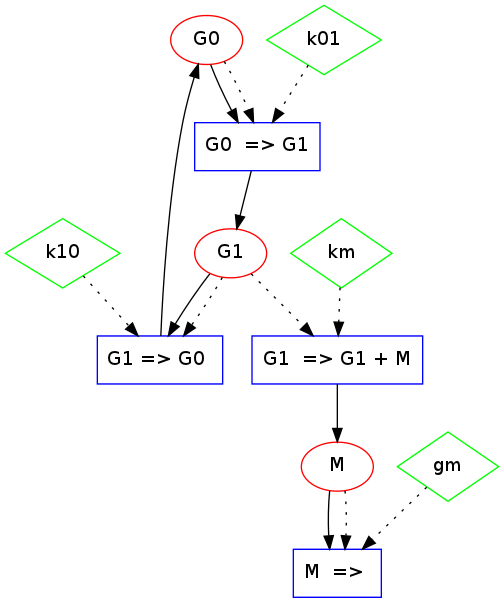
\includegraphics[scale=0.25]{figures/rna1.png}
  \end{minipage}
  \begin{minipage}[b]{0.48\linewidth}
    \centering
    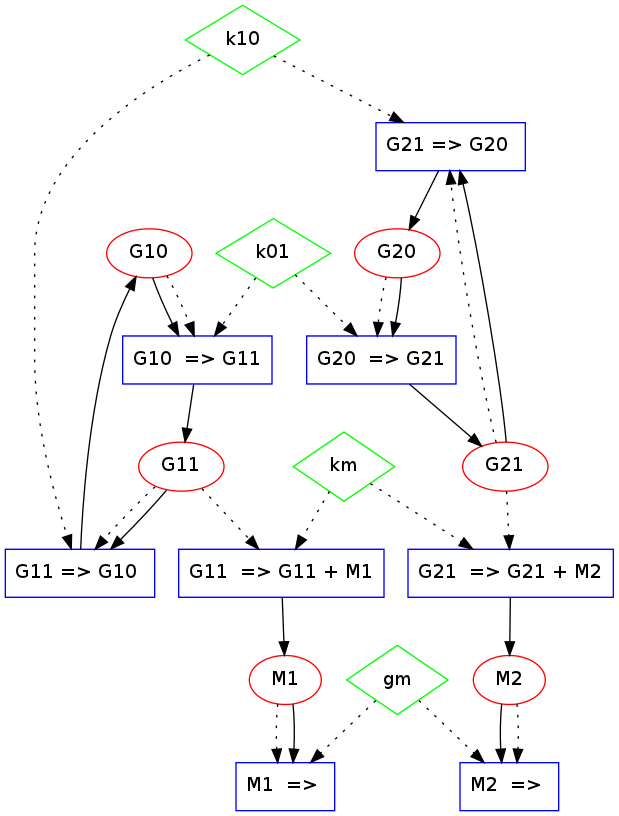
\includegraphics[scale=0.25]{figures/rna2.png}
  \end{minipage}
  \caption{Graph representation of \emph{rna1.rxnm} model (left), and
    \emph{rna2.rxnm} model (right). Species are in red circles,
    parameters in green diamonds, and reactions in blue
    rectangles. Solid arrow represent stoichiometric relations,
    meaning when a reaction consumes or produces a specie. Dotted
    arrows represent rate function dependency, meaning all species and
    parameter that the rate function for a given reaction depends on.}
  \label{fig:rna1dot}
\end{figure}

Now, let's take a look at the simulation specifications. The kinds of
simulations to perform are determined by TYPE attribute. DET
corresponds to deterministic, and SS and ST are stochastic. SS would
keep track of the state of the system at certain time points, and ST
will average the state of the system over certain time
intervals. Further, we have two SCAN options that will be explained later

\subsection{Deterministic Simulation}

We tell the pipeline we want to do a deterministic simulation, with
the TYPE attribute and value DET.  Time points are determined by the
DETPOINTS attribute. All time points values are interpreted the same
as MATLAB syntax. For example
{\footnotesize
\begin{verbatim}
# Example for documentation test1.job
NAME       doc1
OBSERVE    G0,G1,M
TYPE       DET
DETPOINTS  0:100:100000
\end{verbatim}
}
The NAME attribute is a mnemonic string that will be incorporated to
all the output files. The value of OBSERVE is always species symbols
separated by commas. When defined, it will plot the time trajectories
of those species after completing the calculations.

Also, the program will save the results from the simulation into
\textsf{rna1\_doc1\_det.mat} Once completed, located in the
OUTFOLDER. Output file names are constructed using the name of the
model, and the NAME attribute. The variables saved are \\
\begin{tabular}{|p{1.5cm}|p{9cm}|} 
  \hline
  Variable & Description \\
  \hline
  Tdet & time points \\
  Xdet & \#(time points) by \#(species) matrix with the trajectories \\
  XIDs & Cell array with the species symbols \\
  X0 & initial condition \\
  Params & Parameters values \\
  PIDs & Cell array with the species symbols\\
  \hline
\end{tabular}\\ 

When OBSERVE is defined, the figure will
be saved as \emph{rna1\_doc\_det.fig} (see
figure~\ref{fig:test1serie}).

\begin{figure}[H]
  \begin{minipage}[b]{0.48\linewidth}
    \centering
    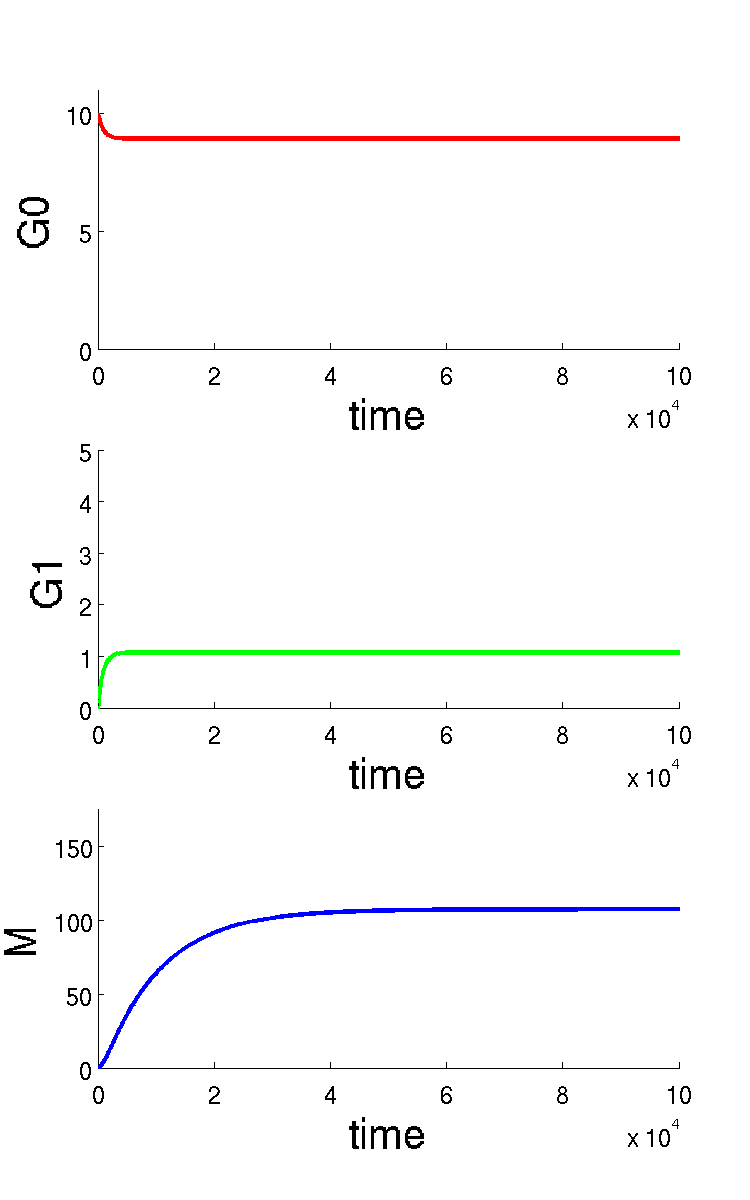
\includegraphics[scale=0.35]{figures/rna1_doc1_det.png}
  \end{minipage}
  \begin{minipage}[b]{0.48\linewidth}
    \centering
    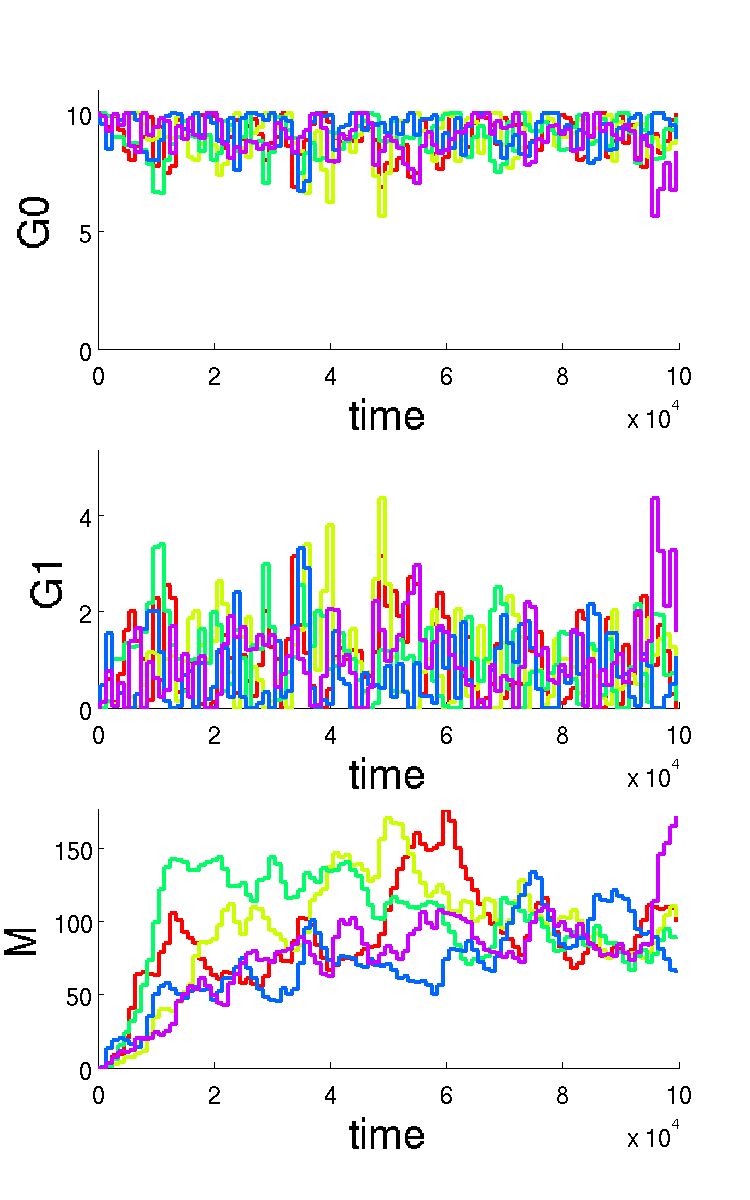
\includegraphics[scale=0.35]{figures/rna1_doc1_st.png}
  \end{minipage}
  \caption{State of the system as a function of time in deterministic
    (left) and stochastic setting (right), as output from
    \textsf{test1.job}. Each colour in the stochastic trajectories
    correspond to a single simulation.}
  \label{fig:test1serie}
\end{figure}

\subsection{Stochastic and Deterministic Compatibility}

We are using a single attribute to store the deterministic rate and
the stochastic propensity of reactions. For this to be consistent,
parameters need to be in units of molecules per cell, instead of molar
concentration, and mechanisms be mass action. Rates different than
mass action may bring inconsistencies. Also, automatically power
functions in rates such as $k*x^2$ will be converted to $k*(1/2)*x*(x-1)$ in
the stochastic setting.

It is important to remember that all units of species are interpreted
as molecules, volume as one cell, and time has arbitrary
units. Meaning it is left to the user to use consistent parameter
values.

\subsection{Stochastic Simulations}

Stochastic simulations have two main attributes the number of times
the simulation will be repeated, and the times points. These are
SSNREP, SSTPOINTS, and STNREP, SSTPOINTS for SS and ST types
respectively. Both stochastic simulations are done in C. MATLAB will
write on the fly the C code, compile it, and execute it. This code
will generate output files, that MATLAB will parse and use to plot the
results.

Time points have a different interpretation on each type.  In SS
simulations, we will keep record of the state of the system at each
time point; whereas for ST simulations, time points will be
interpreted as the limits of time intervals, for which the state of
specie and the square of each specie will be averaged. By default,
initial time will be always recorded.

\subsubsection{Averaging by time intervals}

The way to specify an ST simulation in the \textsf{.job} file is as
{\footnotesize
\begin{verbatim}
# Example for documentation test1.job
TYPE       ST
STNREP     5
STTPOINTS  0:1000:100000
\end{verbatim}
}
For ST simulations, time points will be interpreted as the limits of
time intervals, for which the state of specie and the square of each
specie will be averaged. 

MATLAB will write a C implementation of the simulation
(\textsf{rna1\_doc1\_st.c}), which will save the output in text format
(\textsf{rna1\_doc1\_st...out}), one file per sample. 
{\footnotesize
\begin{verbatim}
0.000000 0.000000 10.000000 0.000000 0.000000 100.000000 0.000000 0.000000
0.000000 1000.000000 10.000000 0.000000 0.000000 100.000000 0.000000 0.000000
1000.000000 2000.000000 10.000000 0.000000 0.000000 100.000000 0.000000 0.000000
2000.000000 3000.000000 9.226512 0.773488 0.961511 90.061027 1.253238 3.970787
3000.000000 4000.000000 9.946531 0.053469 4.000000 133.315626 0.053469 21.493047
4000.000000 5000.000000 10.000000 0.000000 3.343315 395.868282 0.000000 38.031353
...
\end{verbatim}
}
The first and second columns corresponds to the left and right limits
of the time intervals. The file will always begging with $0 0
\ldots$. Then it prints the average state of each species, followed by
the average of the species squared, in the same order. 

Output will be saved in \textsf{.mat} format
(\textsf{rna1\_doc1\_st.mat}) as follow \\
\begin{tabular}{|p{1.5cm}|p{9cm}|} 
  \hline
  Variable & Description \\
  \hline
  Tst & time points interval limits \\
  Xst & Cell array. One matrix for each specie of size \#(time
  intervals) by \#(samples), with the average state of the specie. \\
  X3st & 3 dimensional matrix with the average state of the specie. Size
  \#(time intervals) by \#(species) by \#(samples). \\
  STDst & Cell array. One matrix for each specie of size \#(time
  intervals) by \#(samples), with the standard deviation of the
  state. \\
  STD3st & 3 dimensional matrix with the standard deviation of the
  state. Size \#(time intervals) by \#(species) by \#(samples). \\
  XIDs & Cell array with the species symbols \\
  X0 & Initial states \\
  Params & Parameters values \\
  PIDs & Cell array with the species symbols \\
  \hline
\end{tabular}\\ 

Average trajectory of the species from OBSERVABLE will be plotted, and
saved as \textsf{rna1\_doc1\_st.fig} (see figure~\ref{fig:test1serie}).

\subsubsection{Estimating States Distributions}

In SS simulations, we will keep record of the state of the system at
each time point. The way to specify this in the \textsf{.job} file is
{\footnotesize
\begin{verbatim}
# Example for documentation test1.job
TYPE       SS
SSNREP     2000
SSTPOINTS  1000,10000,100000,500000
\end{verbatim}
}
MATLAB will write a C implementation of the simulation
(\textsf{rna1\_doc1\_ss.c}), which will save the output in text format
(\textsf{rna1\_doc1\_ss.out}).
{\footnotesize
\begin{verbatim}
1000.000000 7 3 6
10000.000000 10 0 88
100000.000000 9 1 56
500000.000000 9 1 91
1000.000000 9 1 5
10000.000000 8 2 31
...
\end{verbatim}
}
The first column are time points, followed by one for each
specie. Notice that the time points are repeated, as we specified more
than one repetition of the simulation.

Output will be saved in \textsf{.mat} format
(\textsf{rna1\_doc\_ss.mat}) as follow \\
\begin{tabular}{|p{1.5cm}|p{9cm}|} 
  \hline
  Variable & Description \\
  \hline
  Tss & time points \\
  Xss & Cell array. One matrix for each specie of size \#(time
  intervals) by \#(samples), with the state of the specie. \\
  X3ss & 3 dimensional matrix with the state of the specie. Size
  \#(time intervals) by \#(species) by \#(samples). \\
  XIDs & Cell array with the species symbols \\
  X0 & Initial states \\
  Params & Parameters values \\
  PIDs & Cell array with the species symbols \\
  \hline
\end{tabular}\\ 

The cumulative frequency of the species states from OBSERVABLE will be
plotted, and saved as \textsf{rna1\_doc1\_ss.fig} (see
figure~\ref{fig:test1dist}).

\begin{figure}[H]
  \centering
  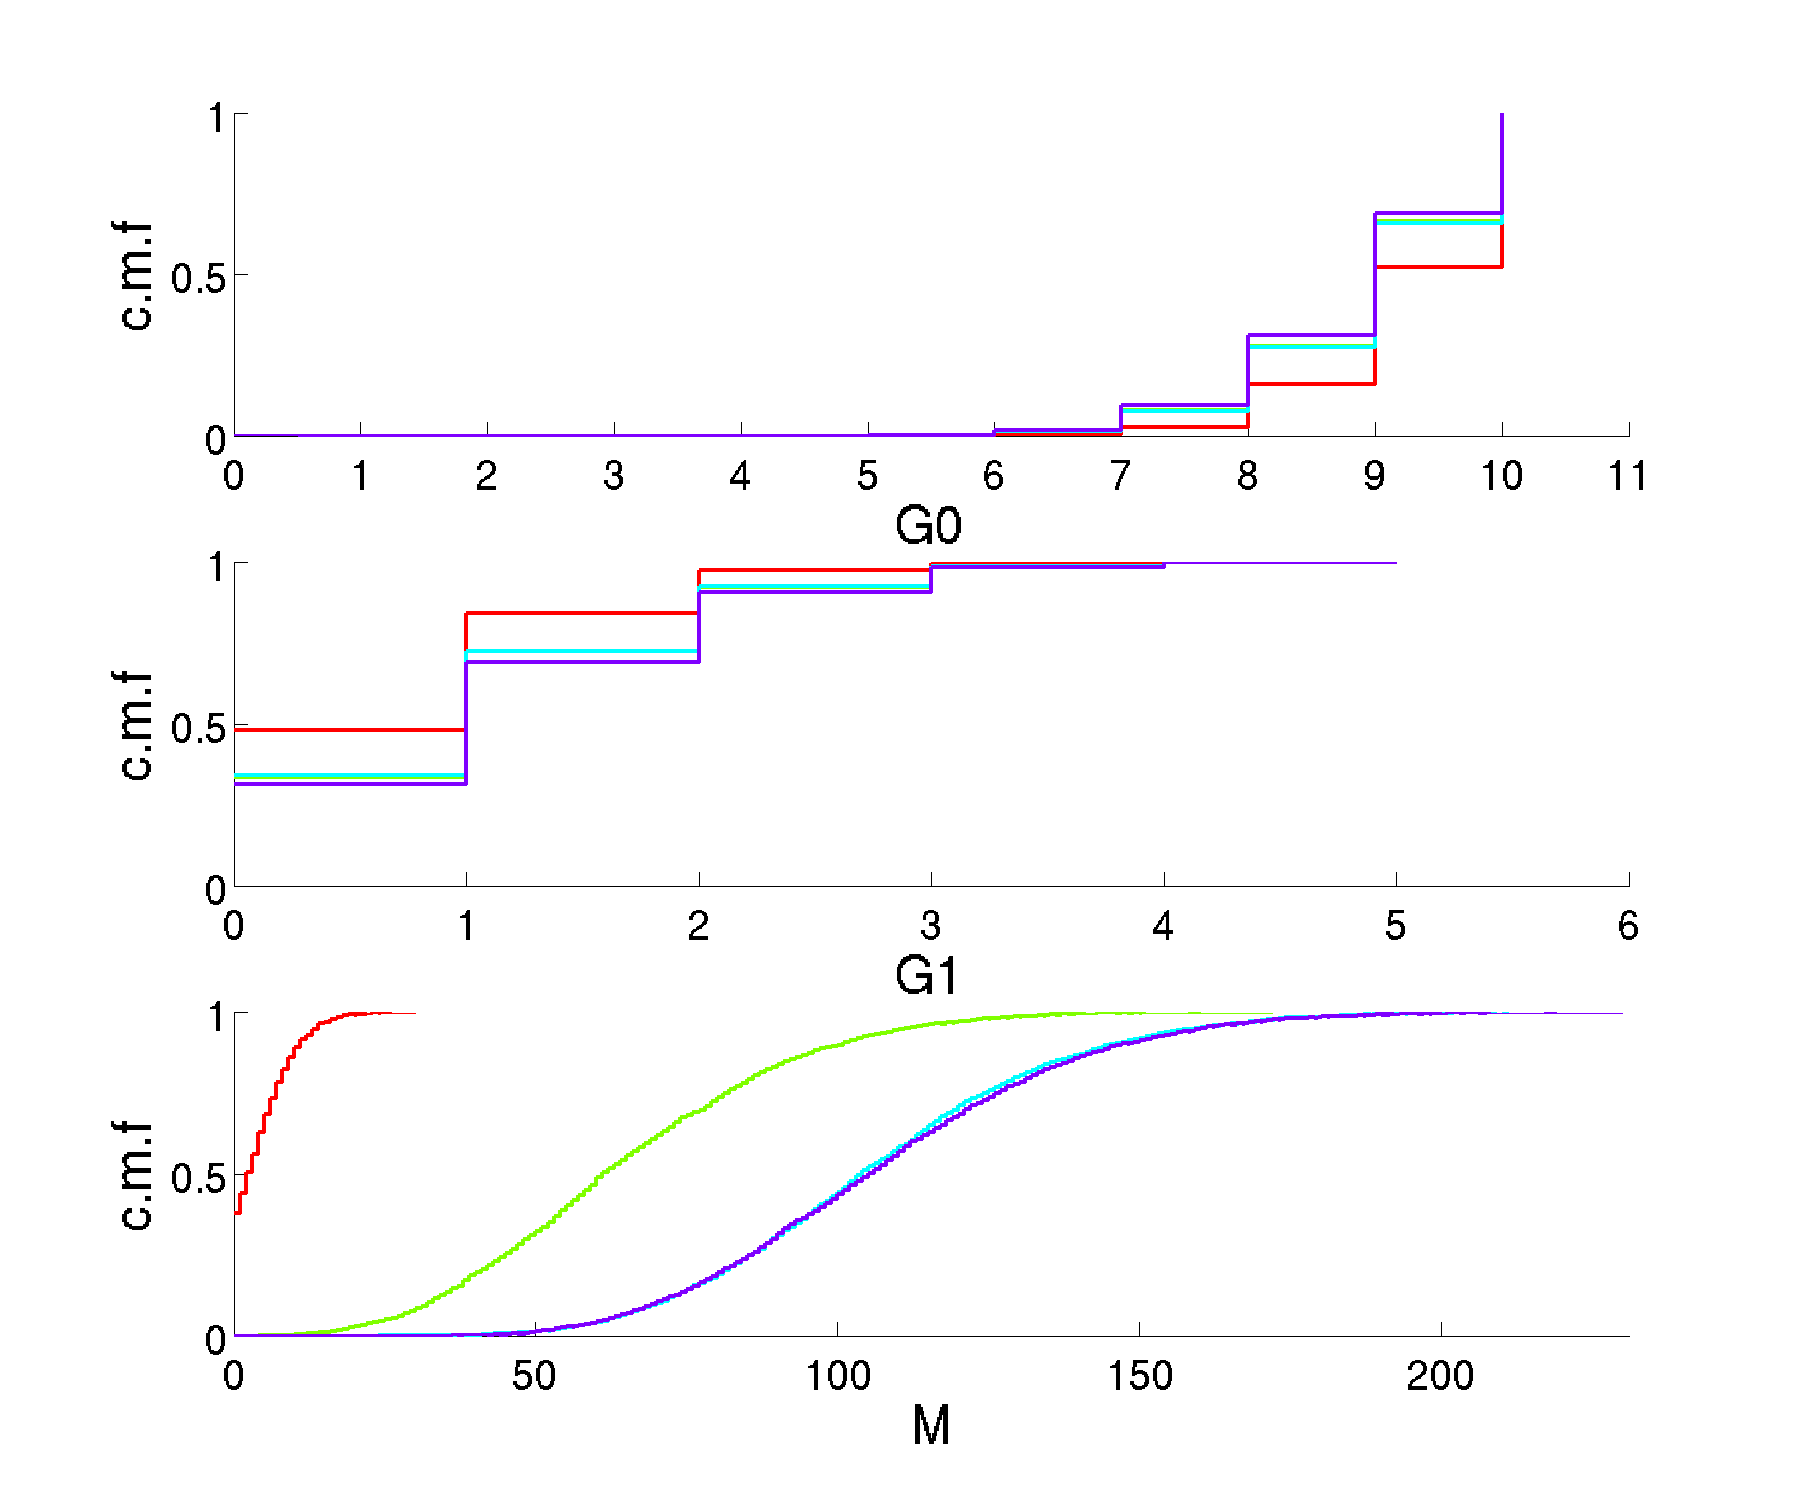
\includegraphics[scale=0.3]{figures/rna1_doc1_ss.png}
  \caption{Cumulative frequency of species states at different time
    points. Each colour corresponds to a single time point.}
  \label{fig:test1dist}
\end{figure}

\subsection{Modifying values from the job file}

It is possible to change the value of parameters and initial states
inside the \emph{.job} file. For example we can set initial state to
20, set parameter $k_m$ to 0.1.
{\footnotesize
\begin{verbatim}
SETINIT    G0:20
SETINIT    km:0.1
\end{verbatim}
}
As a matter of fact, you can add as many IDs as you want separated by
commas before the semicolon, and all of those parameters or species
will be set to that value.

Another feature, is when you have done the simulations, but want to
observe other species. You can prevent from rerunning stochastic
simulations, by changing the figures. For example, if we later become
interested only in the specie M, we add to the \emph{.job} file
{\footnotesize
\begin{verbatim}
OBSERVE    M
NOTSIM     1
\end{verbatim}
}

\subsection{Scatter Plots}

Let's look at a variation of our previous model. We have now two
genes expressing mRNA independently with the very same parameters (see
figure~\ref{fig:rna1dot}).

{\footnotesize
\begin{verbatim}
# Example for documentation test2.job
NAME       doc2
OUTFOLDER  outs2/
MODEL      rna2.rxnm
TYPE       SS
SSNREP     2000
SSTPOINTS  100000
SCATTER    G10,G20
\end{verbatim}
}

Here we have introduced another attribute: SCATTER. The value of this
attribute is a couple or triplet of species IDs separated by commas.
The result, is that a scatter plot with the results from SS type of
simulation will be generated for each time point in SSTPOINTS. The
points will be coloured by the density of values near by that point
(see figure~\ref{fig:scatterG}).

The figure will be saved by appending the names of the variables at
the end \textsf{rna2\_doc2\_ssG10\_vs\_G20.fig}.

\begin{figure}[H]
  \begin{minipage}[b]{0.48\linewidth}
    \centering
    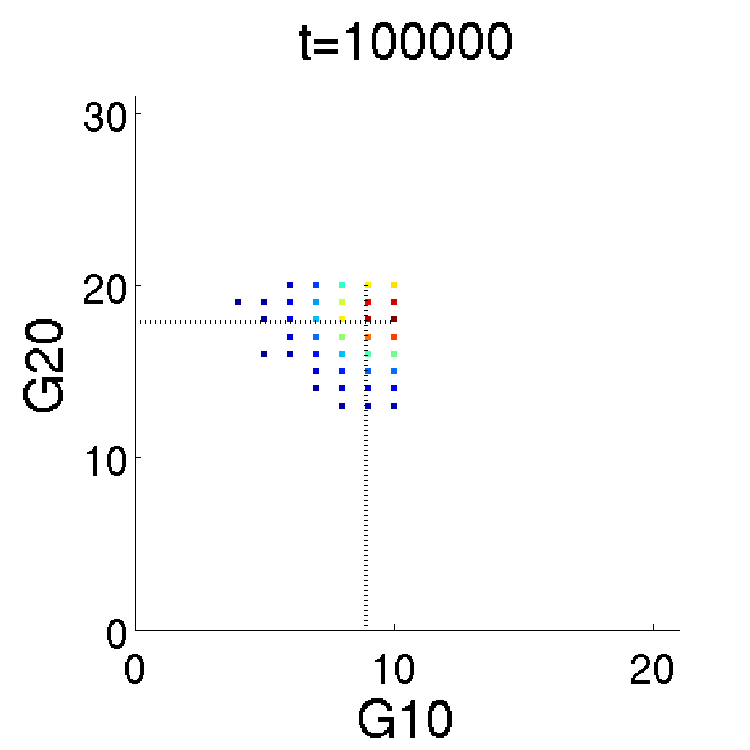
\includegraphics[scale=0.35]{figures/rna2_doc2_ssG10_vs_G20.png}
  \end{minipage}
  \begin{minipage}[b]{0.48\linewidth}
    \centering
    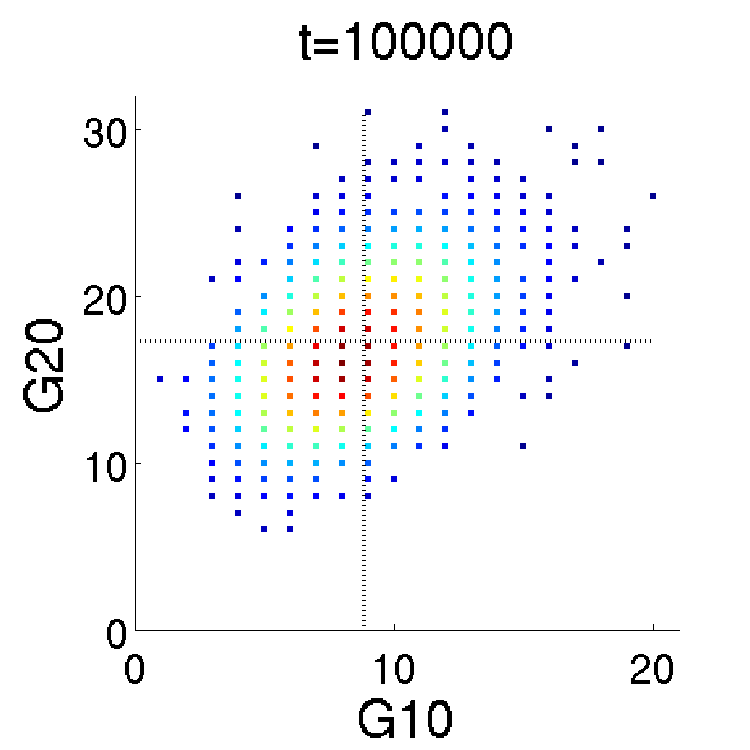
\includegraphics[scale=0.35]{figures/rna2_doc3_ssG10_vs_G20.png}
  \end{minipage}
  \caption{Scatter plots of inactive gene states ($G10$ and
    $G20$). Left case corresponds to a single initial state: 10 and 20
    respectively. On the right, initial state of $G10$ is sampled from
    a Poisson distribution with mean 10, and $G20$ with mean 20. Both
    initial states are correlated with a coefficient of 0.6. Dotted
    lines represent the mean value of each variable.}
  \label{fig:scatterG}
\end{figure}

\subsection{Random initial States and Correlations}

We will work with the model where two genes expressing are mRNA
independently with the very same parameters (see
figure~\ref{fig:rna1dot}).
{\footnotesize
\begin{verbatim}
# First example for documentation test3.job
NAME       doc3
OUTFOLDER  outs3/
MODEL      rna2.rxnm
TYPE       SS
SSNREP     2000
SSTPOINTS  100000
SCATTER    M1,M2
\end{verbatim}
}
Now, say that the initial number of copies of each gene is a random
variable. You can specify that in the \textsf{.job} file.
{\footnotesize
\begin{verbatim}
SETDIST    G10:poiss10.dat
SETDIST    G20:poiss20.dat
\end{verbatim}
}
where \textsf{poiss10.dat} is a text file with two columns, the first
with the values of the variable and second with the \emph{mass density
  function}. In this case, it represents a Poisson distribution with
parameter 10.
{\footnotesize
\begin{verbatim}
0.000000 0.000045
1.000000 0.000454
2.000000 0.002270
...
8.000000 0.112599
9.000000 0.125110
10.000000 0.125110
11.000000 0.113736
12.000000 0.094780
...
\end{verbatim}
}
This will imply that the initial state of $G10$ will be sampled from a
Poisson distribution of mean 10, and $G20$ from a Poisson distribution
of mean 20. Both of these sampling will be independent from one
another. 
The attribute SETDIST is not limited to one specie per time. If many
species share the same distribution we could have added as many
species IDs separated by commas before the semicolon, and all of those
species or species will be sampled from the same distribution.
{\footnotesize
\begin{verbatim}
SETDIST    G10,G20:poiss10.dat
\end{verbatim}
}

If you have a matrix ($M$) in MATLAB structured this way, you can save
it into a file as follow
{\footnotesize
\begin{verbatim}
MATLAB>> savematrix('file.dat',M)
\end{verbatim}
}

To add dependency between the initial states, we specify correlations.
{\footnotesize
\begin{verbatim}
SETCORR    G10,G20:0.6
\end{verbatim}
}
Analogously to SETDIST, we could add many species before the semicolon
and the correlation between all of the them will be set to 0.6.

Example scatter plots comparing the variable and constant initial
states, for the gene inactive states and mRNA are in figures
~\ref{fig:scatterG} and ~\ref{fig:scatterM} respectively.

\begin{figure}[H]
  \begin{minipage}[b]{0.48\linewidth}
    \centering
    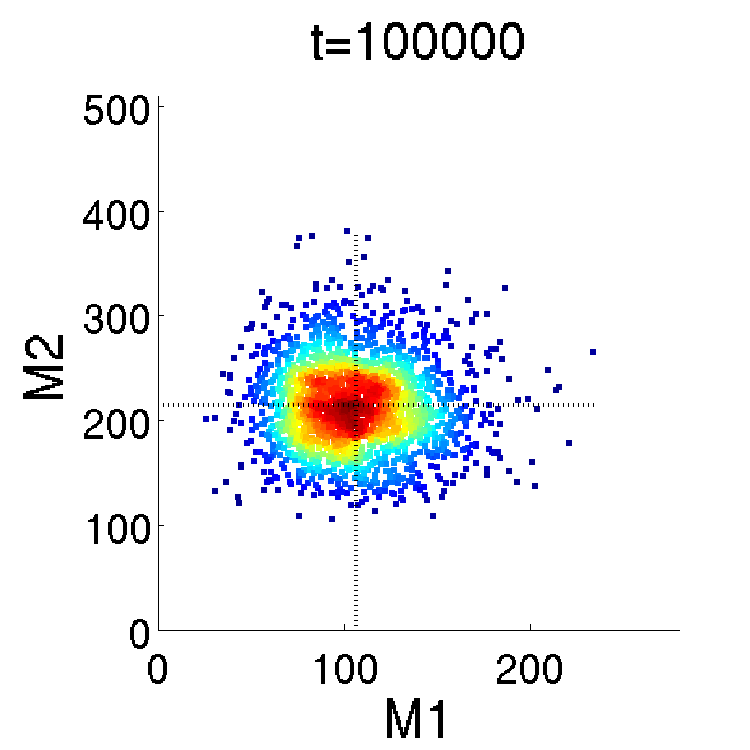
\includegraphics[scale=0.40]{figures/rna2_doc2_ssM1_vs_M2.png}
  \end{minipage}
  \begin{minipage}[b]{0.48\linewidth}
    \centering
    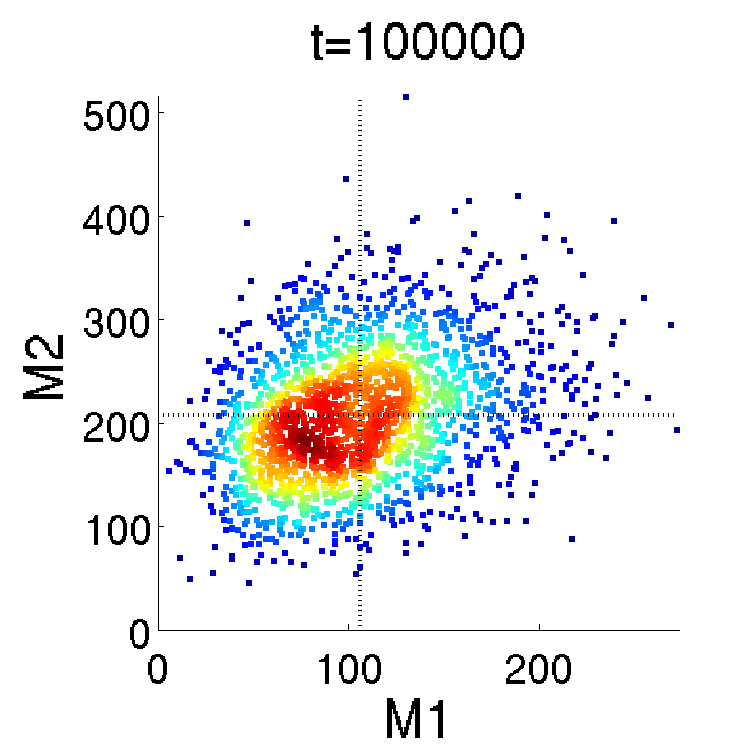
\includegraphics[scale=0.40]{figures/rna2_doc3_ssM1_vs_M2.png}
  \end{minipage}
  \caption{Scatter plots of mRNA expressed from two genes. Initial gene
    copies are deterministic in the right, and random variables in the
    left, as explained in figure~\ref{fig:scatterG}. Dotted lines
    represent the mean value of each variable.}
  \label{fig:scatterM}
\end{figure}

\subsection{Output Scans}

We have implemented shortcuts for exploring the state of the system
under different parameter values and/or initial conditions. There are
under the TYPE values SCANDET and SCANSS. First, we specify the model and
output folder as usual
{\footnotesize
\begin{verbatim}
# Example for documentation test4.job
MODEL      rna2.rxnm # Reaction model
NAME       doc4      # Mnemonic Name
OUTFOLDER  outs4     # Output folder
\end{verbatim}
}

Then, for scanning the values of the system at different gene copy
numbers at time 100000; we use
{\footnotesize
\begin{verbatim}
# Example for documentation test4.job
OBSERVE    M1,M2     # Species for plotting
VARIATE    G10     10:30
VARIATE    G20     10:30
TYPE       SCANDET   # Set scan for deterministic
SCANTIME   100000    # Save the state at that time
\end{verbatim}
}
SCANDET implies that it will use deterministic simulations to estimate
the states, by simulating the system at every combination of values in
VARIATE. VARIATE attribute is defined by two values: a symbol and a
vector. The symbol could be a parameter or specie, where in the later
will be interpreted as variating the initial state of that specie.

The output from the scans will be saved in \textsf{.mat} format
(\textsf{rna1\_doc4\_scandet.mat})\\
\begin{tabular}{|p{1.5cm}|p{9cm}|} 
  \hline
  Variable & Description \\
  \hline
  variate & Symbols of parameters and species that were variated \\
  varvals & A cell array with the values for each symbol in variate \\
  scans & A matrix $n$ by \#(variate), where $n$ is the number of
  combinations bewteen the varvals vectors. Each row corresponds to a
  single combination. \\
  indexes & A matrix the same size as scans, but containing the index
  for each value in the corresponding vector from varvals.\\
  scantime & Time points. By default time 0 is always included to this
  vector. \\
  XscansDET & A 3 dimenstional matrix \#(combinations) by \#(species)
  by \#(time points), containing the state of each specie for each
  combination of parameters. \\
  DefX0 & Default initial states \\
  XIDs & Cell array with the species symbols \\
  DefParams & Default parameter values \\
  PIDs & Cell array with the species symbols \\
  \hline
\end{tabular}\\ 

When OBSERVE is specified, it will plot the values of those species as
a function of the parameters or initial states that were
variated. This is true only for scans of one or two variables (one or
two VARIATE definitions). (See figure ~\ref{fig:scandet}).

\begin{figure}[H]
  \centering
  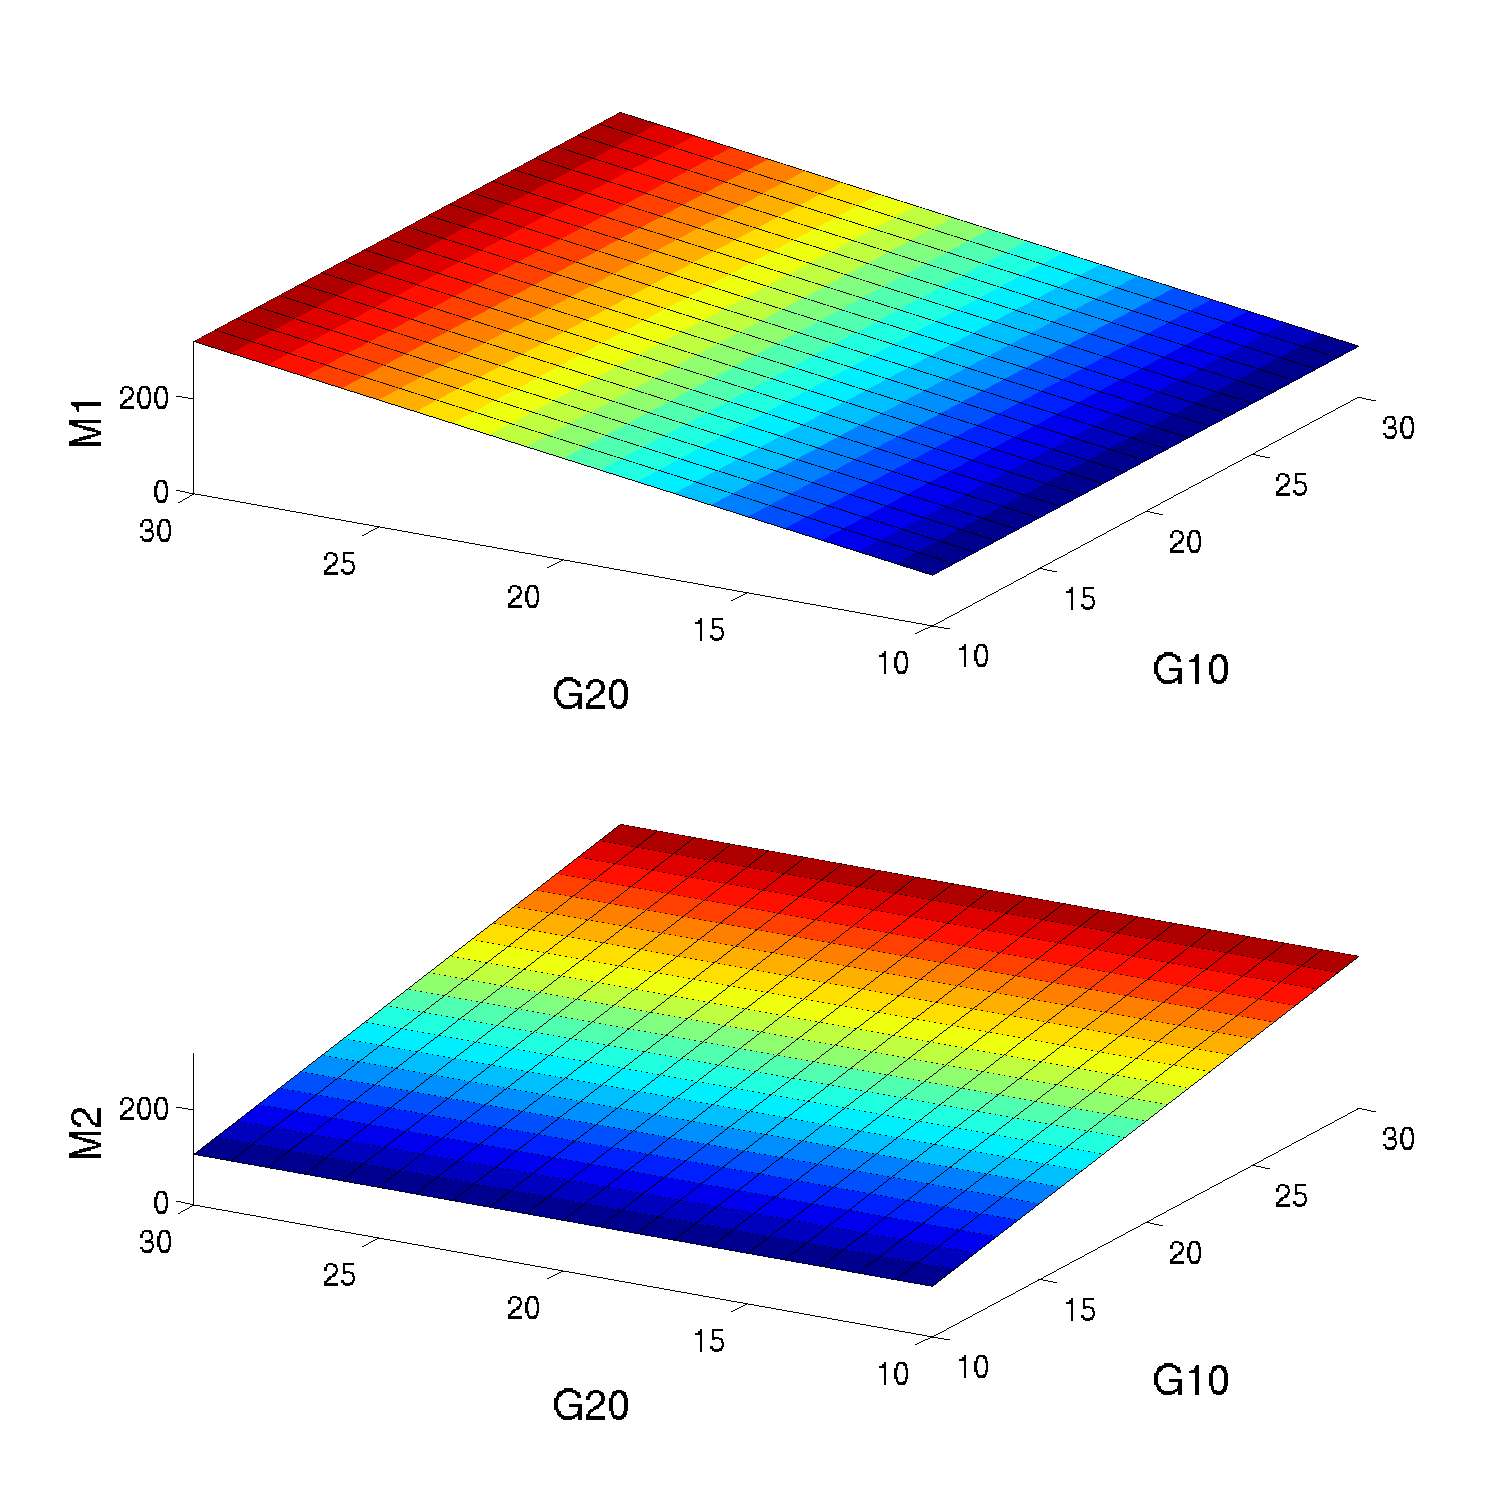
\includegraphics[scale=0.3]{figures/rna2_doc4_scandet_2.png}
  \caption{State of $M1$ and $M2$ at different initial conditions, at
    time 10$^5$. From deterministic simulations.}
  \label{fig:scandet}
\end{figure}

SCANSS is the analogous type, but doing stochastic simulations.
{\footnotesize
\begin{verbatim}
# Example for documentation test4.job
OBSERVE    M1,M2     # Species for plotting
VARIATE    G10     10,20,30
VARIATE    G20     10,20,30
TYPE       SCANSS    # Set scan for stochastc
SCANTIME   100000    # Save the state at that time
SCANREP    50         # Number of samples for stochastic simulations
\end{verbatim}
}
SCANREP specifies how many samples are computed at each combination of
the VARIATE vectors.

The output from the scans will be saved in \textsf{.mat} format
(\textsf{rna1\_doc4\_scanss.mat}) \\
\begin{tabular}{|p{1.5cm}|p{9cm}|} 
  \hline
  Variable & Description \\
  \hline
  variate & Symbols of parameters and species that were variated \\
  varvals & A cell array with the values for each symbol in variate \\
  scans & A matrix $n$ by \#(variate), where $n$ is the number of
  combinations between the varvals vectors. Each row corresponds to a
  single combination. \\
  indexes & A matrix the same size as scans, but containing the index
  for each value in the corresponding vector from varvals.\\
  scantime & Time points. By default time 0 is always included to this
  vector. \\
  XscansSS & A cell array, with 3 dimensional matrices
  \#(combinations) by \#(species) by \#(samples) with a vector the
  states in all samples at final scantime \\
  scans3 & A matrix \#(combinations)*\#(samples) by \#(variate), where
  each row of scan has been repeated \#(samples) times.\\
  indexes3 & A matrix \#(combinations)*\#(samples) by \#(variate),
  where each row of indexes has been repeated \#(samples) times.\\
  X3scansSS & A 3 dimensional Matrix \#(combinations)*\#(samples) by
  \#(species) by \#(time points) containing the states at each time
  point and condition. The rows in the first dimension correspond to
  the conditions in scan3. \\
  X4scansSS & A 4 dimensional Matrix \#(combinations) by \#(species)
  by \#(time points) by \#(samples) containing the states at each time
  point and condition. \\
  DefX0 & Default initial states \\
  XIDs & Cell array with the species symbols \\
  DefParams & Default parameter values \\
  PIDs & Cell array with the species symbols \\
  \hline
\end{tabular}\\ 

When OBSERVE is specified, it will plot the average and coefficient of
variation of those species as a function of the parameters or initial
states that were variated. This is true only for scans of one or two
variables (one or two VARIATE definitions). (See figure
~\ref{fig:scanss})

\begin{figure}[H]
  \centering
  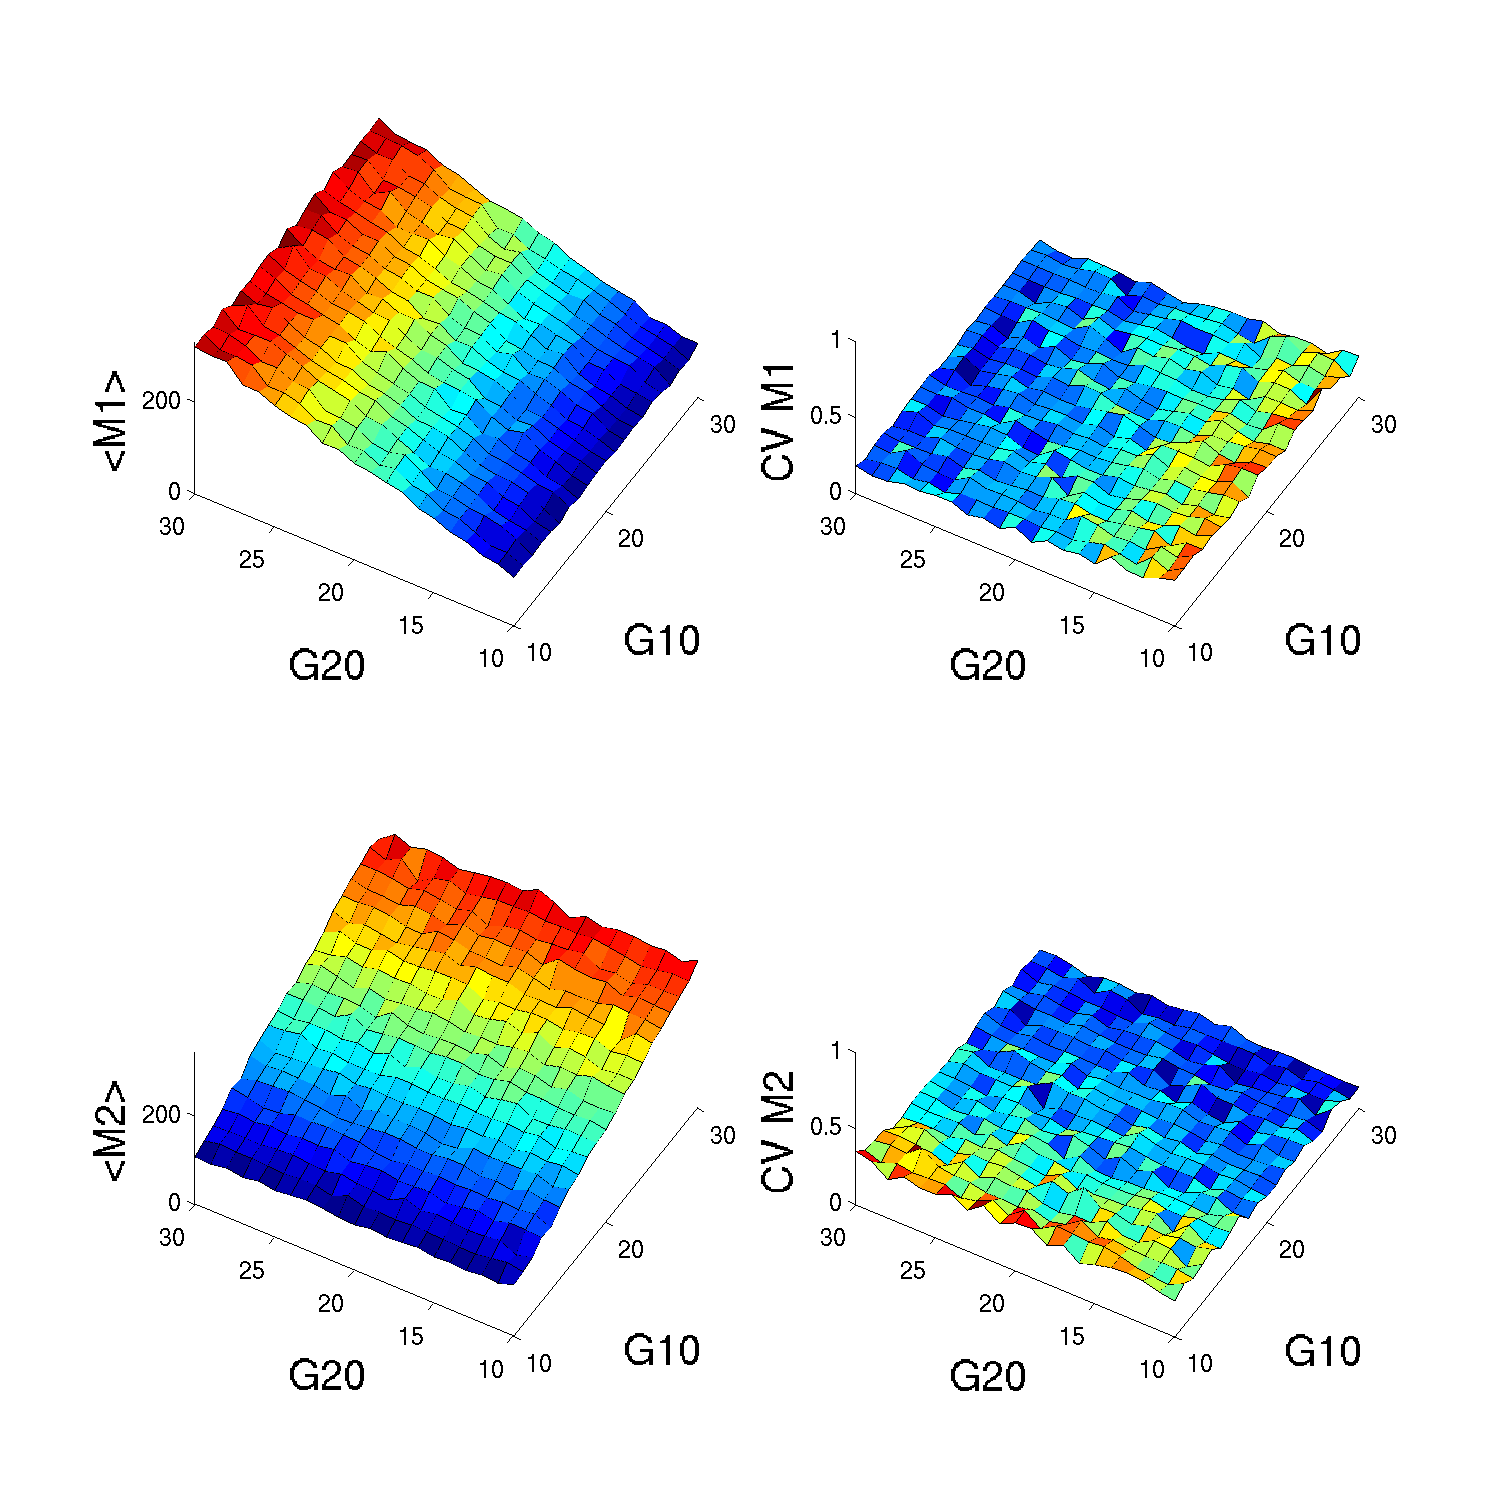
\includegraphics[scale=0.4]{figures/rna2_doc4_scanss_2.png}
  \caption{Average and CV of $M1$ and $M2$ copy numbers at different
    initial conditions, at time 10$^5$. From Stochastic Simulations.}
  \label{fig:scanss}
\end{figure}

\section{Future Improvements}

Some of the next steps that could improve these tools could be:
\begin{itemize}
\item Implement Gibson and Brucks stochastic method \citep{Gibson2000}.
\item Implement scans in C.
\item Instead of writing our own C code, make it compatible with
  MATLAB C compiler. Then we could pass variables directly.
\item Use parallel computing.

\item Do unit checking before compiling.
\item Implement parameters as random variables.
\item Explicitly include volume and do corrections in the fly. How to
  handle non mass action rates is an open question to me.

\end{itemize}

\footnotesize
\bibliographystyle{plain}
\bibliography{references}

\end{document}
